% senior_thesis-proposal.tex
% Gregory M. Kapfhammer
% CMPSC 580, Spring 2013
%
% Revised by R. Roos
% Sep 2013
%
% This document provides a sample senior thesis proposal template for use
% by students in Allegheny's CS and Applied Computing programs.
%
%   *******************************************************************
%   * LOOK FOR BLOCK COMMENTS SUCH AS THIS ONE FOR AN EXPLANATION OF  *
%   * THIS DOCUMENT AND HOW TO MODIFY IT FOR YOUR OWN PROPOSAL!       *
%   *                                                                 *
%   * ANY LINE BEGINNING WITH A "%" IS A LATEX COMMENT AND IS IGNORED *
%   * BY THE LATEX PROCESSOR. YOU ARE ENCOURAGED TO COMMENT YOUR OWN  *
%   * LATEX CODE.                                                     *
%   *******************************************************************

%   ********************************************************************
%   * THE FIRST SECTION OF THE LATEX FILE IS THE "PREAMBLE." IT        *
%   * INSTRUCTS LATEX TO IMPORT SPECIAL PACKAGES FOR THINGS LIKE       *
%   * INCLUDING FIGURES, DOUBLE-SPACING, COLORED TEXT, ETC.            *
%   * DEPENDING ON YOUR NEEDS, YOU MAY FIND IT NECESSARY TO USE PACK-  *
%   * AGES THAT ARE NOT INCLUDED IN THIS TEMPLATE. SIMPLY IMITATE THE  *
%   * "\usepackage{...}" COMMANDS SHOWN BELOW.                         *
%   ***************\begin{Huge}
%   *****************************************************

%   ********************************************************************
%   * BEGINNING OF PREAMBLE:                                           *
%   ********************************************************************
\documentclass[11pt]{article}


\topmargin 0.0in
\setlength{\textwidth} {420pt}
\setlength{\textheight} {620pt} 
\setlength{\oddsidemargin} {20pt}
\setlength{\marginparwidth} {72in}

\usepackage[T1]{fontenc}
\usepackage{mathptmx}
\usepackage{fancyhdr} 
\usepackage{url}
\usepackage{graphicx}
\usepackage{tikz}
\usepackage{listings}
\usepackage{color}
\usepackage{tikzpagenodes}
\usepackage{lipsum}
\usepackage{capt-of}
\usepackage{floatrow}
\usepackage{subfig}
\usepackage[latin1]{inputenc}


\floatsetup[figure]{style=plain,subcapbesideposition=center}

\definecolor{dkgreen}{rgb}{0,0.6,0}
\definecolor{gray}{rgb}{0.5,0.5,0.5}
\definecolor{mauve}{rgb}{0.58,0,0.82}

\lstset{frame=tb,
  language=Java,
  aboveskip=3mm,
  belowskip=3mm,
  showstringspaces=false,
  columns=flexible,
  basicstyle={\small\ttfamily},
  numbers=none,
  numberstyle=\tiny\color{gray},
  keywordstyle=\color{blue},
  commentstyle=\color{dkgreen},
  stringstyle=\color{mauve},
  breaklines=true,
  breakatwhitespace=true,
  tabsize=3
}

\usepackage{setspace}
\usetikzlibrary{calc,trees,positioning,arrows,chains,shapes.geometric,%
    decorations.pathreplacing,decorations.pathmorphing,shapes,%
    matrix,shapes.symbols,fit}
    
\tikzstyle{decision} = [diamond, draw, fill=blue!20, 
    text width=4.5em, text badly centered, node distance=3cm, inner sep=0pt]
\tikzstyle{block} = [rectangle, draw, fill=blue!20, 
    text width=5em, text centered, rounded corners, minimum height=4em]
\tikzstyle{line} = [draw, -latex']
\tikzstyle{cloud} = [draw, ellipse,fill=red!20, node distance=3cm,
    minimum height=2em]

\tikzset{
%>=stealth',
  punktchain/.style={
    rectangle, 
    rounded corners, 
    % fill=black!10,
    draw=orange, very thick,
    text width=10em, 
    minimum height=1em, 
    text centered, 
    on chain},
  line/.style={draw, thick, <-},
  element/.style={
    tape,
    top color=white,
    bottom color=blue!50!black!60!,
   minimum width=8em,
    draw=blue!40!black!90, very thick,
    text width=10em, 
    minimum height=1em, 
    text centered, 
    on chain},
  every join/.style={->, thick,shorten >=1pt},
  decoration={brace},
  tuborg/.style={decorate},
  tubnode/.style={midway, right=2pt},
}
% set it so that subsubsections have numbers and they
% are displayed in the TOC (maybe hard to read, might want to disable)

\setcounter{secnumdepth}{3}
\setcounter{tocdepth}{3}

% define widow protection

\def\widow#1{\vskip #1\vbadness10000\penalty-200\vskip-#1}

\clubpenalty=10000  % Don't allow orphans
\widowpenalty=10000 % Don't allow widows

% this should give me the ability to use some math symbols that 
% were available by default in standard latex (i.e. \Box)

\usepackage{latexsym}

% define a little section heading that doesn't go with any number

\def\littlesection#1{
\widow{2cm}
\vskip 0.5cm
\noindent{\bf #1}
\vskip 0.0001cm 
}

\pagestyle{fancyplain}

\newcommand{\tstamp}{\today}   
\renewcommand{\sectionmark}[1]{\markright{#1}}
\lhead[\Section \thesection]            {\fancyplain{}{\rightmark}}
\chead[\fancyplain{}{}]                 {\fancyplain{}{}}
\rhead[\fancyplain{}{\rightmark}]       {\fancyplain{}{\thepage}}
\cfoot[\fancyplain{\thepage}{}]         {\fancyplain{\thepage}{}}

\newlength{\myVSpace}% the height of the box
\setlength{\myVSpace}{1ex}% the default, 
\newcommand\xstrut{\raisebox{-.5\myVSpace}% symmetric behaviour, 
  {\rule{0pt}{\myVSpace}}%
}

% leave things with no spacing extra spacing in the final version of the paper
\renewcommand{\baselinestretch}{1.0}    % must go before the begin of doc

% suppress the use of indentation for a paragraph

\setlength{\parindent}{0.0in}
\setlength{\parskip}{0.1in}

\begin{document}
\doublespacing

% handle widows appropriately
\def\widow#1{\vskip #1\vbadness10000\penalty-200\vskip-#1}

% build the title section

\makeatletter

\def\maketitle{%
  %\null
  \thispagestyle{empty}%
  %\vfill
  \begin{center}%\leavevmode
    %\normalfont
    {\Huge \@title\par}%
    %\hrulefill\par
    {\normalsize \@author\par}%
    \vskip .4in
%    {\Large \@date\par}%
  \end{center}%
  %\vfill
  %\null
  %\cleardoublepage

  }

\makeatother

%   ********************************************************************
%   * Here is the first place where you need to begin customizing:     *
%   * Enter you name, the title of your proposal, etc., in the places  *
%   * indicated by the comment "% CHANGE!".                            *
%   ********************************************************************

\vspace*{-1.1in}
\title{Empirical Study of Tools to Assist Java Programmers in Finding Bugs}  % CHANGE!

% build the author section
\author{
        Andreas Landgrebe\\  % CHANGE!
        Department of Computer Science\\
        Allegheny College \\
        {\tt landgrebea@allegheny.edu}  \\  % CHANGE!
        \vspace*{.1in} \today \\ \vspace*{.1in}
}

\maketitle       % use the default title stuff

% Default "abstract" environment is too small; customize one instead:
\begin{center}
\large\bf Abstract
\vspace{-1em}  % Reduce space between header and the abstract
\end{center}

%   ********************************************************************
%   * Here is the second place where you need to customize:            *
%   * enter your abstract in the "quote" environment:                 *
%   ********************************************************************

\begin{quote}

As a programmer, it is inevitable to encounter logic based bugs and it is imperative to be able to fix these issues. One approach to this situation is to find tools that detects these bugs. Tools will assist programmers to they can spend time on different parts of a project rather than trying to find a bug. This paper presents a empirical study to further examine the  tools Findbugs, PMD, and Checkstyle used to find logic based bugs are found in the Java programming language. 
%Provide a concise summary of your proposed research. Remember that
%the abstract is {\it not} an introduction, it is a {\it summary} of the
%entire document. It makes sense to wait to write the abstract until the
%rest of the document has been written.
\end{quote}

%\vspace*{-.4in}
\section{Introduction}
\label{sec:introduction}
\vspace*{-.1in}

%   ********************************************************************
%   * Enter the text of your introductory section here.                *

%   ********************************************************************
\subsection{Motivation}

%Provide an intuitive motivation for and introduction to your proposed
%senior thesis research.  Whenever possible, you should use one or more
%concrete examples and technical diagrams.

As one writes in the Java programming language, there will be a high chance that programs will not run as expected. In order to resolve such a problem, there are many options to fix the issue. One approach is to look back into the source code and read line-by-line and try to find out what the issue is. This approach is time consuming and tiresome and may not always work. An alternative approach is to use a tool such as Findbugs, PMD, or Checkstyle to find the issue.

\begin{figure}%[htbp]
\sidesubfloat[]{
\begin{tikzpicture}
  [node distance=.2cm,
  start chain=going below,]
     \node[punktchain, join](HighCard){High Card};
     \node[punktchain, join](OnePair){One Pair};
     \node[punktchain, join](TwoPair){Two Pair};
     \node[punktchain, join](ThreeofaKind){Three of a Kind};
     \node[punktchain, join](Straight){Straight};
     \node[punktchain, join](Flush){Flush};
     \node[punktchain, join] (FullHouse){Full House};
     \node[punktchain, join] (FourofaKind){Four of a Kind};
     \node[punktchain, join] (StraightFlush){Straight Flush};
     \node[punktchain, join] (RoyalFlush) {Royal Flush}; 

   \end{tikzpicture}
	
}\qquad
\sidesubfloat[]{
\begin{tikzpicture}
  [node distance=.2cm,
  start chain=going below,]
     \node[punktchain, join] (RoyalFlush) {Royal Flush};
     \node[punktchain, join] (StraightFlush){Straight Flush};
     \node[punktchain, join] (FourofaKind){Four of a Kind};
     \node[punktchain, join] (FullHouse){Full House};
     \node[punktchain, join](Flush){Flush};
     \node[punktchain, join](Straight){Straight};
     \node[punktchain, join](ThreeofaKind){Three of a Kind};
     \node[punktchain, join](TwoPair){Two Pair};
     \node[punktchain, join](OnePair){One Pair};
     \node[punktchain, join](HighCard){High Card};

   \end{tikzpicture}
   }
   \caption{(a) shows the wrong representation and (b) shows the correct representation to follow when playing a game of poker}
   \label{fig:pr}
   \end{figure}
   
\newpage

For example, lets say we are developing a game of poker in Java code. Figure \ref{fig:pr} shows different poker hands that a player can have. Figure \ref{fig:pr} (a) shows the wrong representation and Figure \ref{fig:pr} (b) shows the correct representation on how to follow a game of poker. Figure \ref{fig:pr} (a) would be a wrong because a program is looking for a hand that contains a pair before they look for a hand that could possibly have two pairs inside it. Therefore this design will not select the highest possible combination. To fix this, Figure \ref{fig:pr} (b) would be the correct representation of how a game of poker should be played. The tools of Findbugs, PMD and Checkstyle will be evaluated to see if they ciouyld suggest the big is in the sequence of the poker hand representation.

\subsection{Definition}


Static program analysis is defined as analysis of software that is completed without actually executing programs. This type of analysis is usually perform as part of a Code Review. This analysis attempts to highlight possible errors within non-running source code. An example of this is the three tools Findbugs, PMD, and Checkstyle. These tools checks for faults in the Java program without the Java program running. Static program analysis tools are grouped into four types. The first one is a code analysis where statements can be highlighted if the syntax is wrong. the next group is the structure checker. This group of tools generates a graph from the components submitted as input. The next group is called data analyzers. This group of tools reviews the data structures and then notes improper linkage among components. The last group is called the sequence checker. This group of tools checkes sequences of events. If the program is coded in the incorrect sequence, the events are highlighted.

Dynamic Program Analysis is defined as the analysis of computer software that is performed by executing programs on a real or virtual processor. These tools are also known as program monitors because they watch and report the program's behavior. 

Fault of omission is defined as one that results when some key aspect of the code is missing. For example, a fault may occur when a variable is not initialized.

Fault of commission is defined as a fault in a program that is incorrect. For example, the variable is initialized to the wrong value.


 Logic-based bug is defined as a bug in a program that causes it operate incorrectly, but not to terminate abnormally or crash. This is considered to be fault of comission. An example of a logic-based bug is say you have a program that is supposed to calculate velocity squared. Velocity squared should equal $2 * (kinetic / mass).$ But instead, your program is calculating Velocity squared to be $3 * (kinetic / mass).$ Now due to the fact that it is not following the law of physics, this is considered to be a logic-based bug. 

 Compiler bug is a defined as a bug in a program that prevents it from running. This is considered to be a fault of omission. An example of a compiler bug is using a variable such as $x$ throughout a Java program but you initialize it.

 Run-time bug is defined as a bug in a program that occurs during the execution of a program. Contrast to logic-based bugs, run-time bugs will terminate or crash. 

 False Positive is defined as an error in data reporting in which a test result improperly indicates presence of a condition. The result of this is positive. An example of this is if one uses the tool Findbugs, PMD, or Checkstyle. These tools could report a false positive if they scan through source code and highlights a line of source code that that is not actually a bug in the program. 

 False Negative is defined as an errors in which a test result improperly indicates no presence of a conditions. The result in this case will be negative. An example of this is if one uses the tool Findbugs, PMD, or Checkstyle. These tools could report a false negative if they scan through source code and after going through a program, the tools were not able to highlight a line of source code and according to the tool, the program does not have any bug when the program does hold a bug.


 Cyclomatic Complexity is defined as a software measurement used to indicate the complexity of a program. This measurement metric calculate the number of linearly independent paths through a program's source code. A tools such as PMD is able to detect the complexity of a program by calculauting the amount of linearly independent paths are in a program's source code.

 Inefficient Code is defined as looking at a program and noticing it can be re-written to be simpler. One example of inefficient code in the Java programming language is when checking a string to see if it is empty. Using the String.trim().length() would be considered to be an inefficient approach to check if a string is empty. this is due to the fact that this approach creates a new String object just to check its size. Instead consider creating a static function that loops through the string. This would be a much more efficient approach to checking to see if a string is empty. 




\vspace*{-.1in}
\section{Related Work}
\label{sec:relatedwork}
\vspace*{-.1in}

 Automated and semi-automated analysis of source code has remained a topic of intense research for more than 30 years\cite{Binkley}. In this paper, it provides future predictions of source code analysis, applications, and techniques that will be in development. This paper also provides a definition of what source code analysis is. ``Source code analysis is the process of extracting information about a program from its source code or artifacts generated from the source code using automatic tools \cite{Binkley}." The idea of source code analysis is imperative in order to figure how a programs works. Source code analysis is also used to locate bugs in programs. Using  source code analysis to implement this tool is one of the main ideas for this proposed senior project. 


\begin{table}[htbp]
\begin{tabular}{|c|c|c|}
\hline
\includegraphics[scale=0.5]{JavaVisualizer}
\end{tabular}
\caption{Java Visualizer being used to go through a Java program line by line}
\label{tab:jv}
\end{table}

In Table \ref{tab:jv}, the Java Visualizer is used to go through a Java program line by line and  have a visualization of the program on the right hand side.

Despite all of the related work that has been implemented, there are quite a few flaws that have been noticed. The tools that are presented in this paper may not detect a possible bug or may highlight a point in the source code that may not be the bug. My proposed study is to evaluate three tools for five Java programs that have been written and include a bug. This will provide Java programmers information about possibly detecting logic based bugs.

\vspace*{-.1in}
\section{Tools}
\label{sec:tools}
\vspace*{-.1in}

\subsection{Findbugs}

FindBugs is an open-source tool that uses static analysis to detect logic-based bugs in Java code \cite{BugFindingTools}. It will tell the programmer where the bugs most likely will be. Being able to provide as much information to the programmer to be able to debug a Java program is imperative for programming. Findbugs will not give the programmer the exact location of the bug. This program looks for instances of bug patterns so it will highlights code instances that are likely to be errors. This tools ranks potential bugs in four categories. (i) is the scariest, (ii) is scary, (iii) is troubling, and (iv) is a concern. This gives the programmer a possible hit as to where a bug may be in the program. Findbugs operates on Java bytecode rather than source code. This proves that Findbugs cannot be used if one is having compiler issues. This tool can be used to detect a possible run time issue.  
\newpage
\begin{table}[htbp]
\begin{tabular}{|c||c|c|}
\hline
\includegraphics[scale=0.45]{findbugs1}
\end{tabular}
\caption{Findbugs used in the Eclipse environment}
\label{tab:fb}
\end{table}

In Table \ref{tab:fb}, the Findbugs tool is being used in the Eclipse Integrated Development Environment. As shown in  the figure, Findbugs is able to analyze source code line by line and display where the most troubling code is. This tool may not find the exact bug in a particular piece of source code but it assists the programmer by advising where the bug may be in a Java program.


\subsection{PMD}

PMD is a source code analyzer. Unlike Findbugs that looks for bugs at the Java bytecode level, PMD search for possible bugs at the source code level. PMD scans Java source code and look for potential problems such as  dead code, suboptimal code, overcomplicated expressions, and duplicate code \cite{BugFindingTools}. This tool includes a set of built-in rules and supports the ability to write custom rules. Most of the time, PMD will report issues based on of inefficient code. 
\begin{table}[htbp]
\begin{tabular}{|c||c|c|}
\hline
\centering
\includegraphics[scale=0.45]{eclipse-pmdmarkers.png}
\end{tabular}
\caption{Example of PMD used in the Eclipse Integrated Development Environment}
\label{tab:PMD}
\end{table}

\newpage

\subsection{Checkstyle}

Checkstyle is a development tools to help programmer write Java code that adheres to a coding standard \cite{Merson:2013:UAE:2508075.2508433}. This is also a static code analysis tool used in software development such as Findbugs and PMD. Checkstyle checks at the Java source code level to see if it complies with coding rules set upon. 

\begin{table}[htbp]
\begin{tabular}{|c||c|c|}
\hline
\includegraphics[scale=0.45]{15466.png}
\end{tabular}
\caption{Example of checkstyle being used in the Eclipse Integrated Development Environment}
\label{intro-fig3}
\end{table}








%   ********************************************************************
%   * Enter the text of your related work section here.                *
%   ********************************************************************

%Summarize the previously published papers and books that are related
%to your proposed research.  Whenever possible, you should compare and
%constrast your approach with the ones that have been discussed in the
%past.  As you describe your papers, please make sure that you cite
%them properly \cite{conrad-gecco-selection-study}.

%   ********************************************************************
%   * Enter the text of your method of approach section here.          *
%   ********************************************************************

%Use technical diagrams, equations, algorithms, and paragraphs of text
%to describe the research that you intend to complete. See the \LaTeX\ source
%file for the proposal to learn how Figure \ref{intro-fig1} and Table 

%explicitly refer to them in your text.

\vspace*{-.2in}
\section{Evaluation Strategy}
\label{sec:evaluate}
\vspace*{-.1in}

%   ********************************************************************
%   * Enter the text of your evaluation strategy section here.         *
After these tools have been analyzed, the next step for this senior project is  to give a empirical study to students in the classes of Computer Science 112 and more advanced classes at Allegheny College. Doing so, this will allow me to see the effective of the examined tools. The results will tell me if students in Computer Science 112 and other classes were able to fix issues they were having or if they were better off reading source code line to line to debug code.  

In order to give the best results, all students in Computer Science 112 will use the tools to see if they assist in finding  bugs in the Java programs. There should be at least 20 students. After the students have evaluated the tools, anyone with a basic knowledge of Java programming past Computer Science 111 can be used for the empirical study. Ideally, in order to have the best results, a empirical study of at least 40 people would provide the best results. Students will be using the Eclipse Integrated Development Environment which will have the three tools Findbugs, PMD and Checkstyle added to be evaluated. 
\newpage
\begin{figure}
\begin{tikzpicture}[node distance = 2.6cm]
    % Place nodes
    \node [block] (startTrial) {Start Trial};
    \node [block, below of=startTrial] (javaBuggyProgram) {Java Buggy Program};
    \node [block, below of=javaBuggyProgram] (toolOne) {Tool A};
    \node [block, left of=javaBuggyProgram] (yesOne) {Yes};
    \node [block, right of=toolOne] (noOne) {No};
    \node[block, below of=noOne] (toolTwo) {Tool B};
    \node[block, left of=yesOne] (yesTwo) {Yes};
    \node[block, right of=toolTwo] (noTwo) {No};
    \node[block, below of=noTwo] (toolThree) {Tool C};
    \node[block, left of=yesTwo](lastYesNo) {Yes or No};
    % Draw edges
    \path [line] (javaBuggyProgram) -- (startTrial);
    \path [line] (toolOne) -- (javaBuggyProgram);
    \path [line] (yesOne) |- (toolOne);
    \path [line] (noOne) -- (toolOne);
    \path [line] (startTrial) -| (yesOne); 
    \path [line] (toolTwo) -- (noOne);
    \path [line] (yesTwo) |- (toolTwo);
    \path [line] (noTwo) -- (toolTwo);
    \path [line] (startTrial) -| (yesTwo);
    \path [line] (toolThree) -- (noTwo);
    \path [line] (lastYesNo) |- (toolThree);
    \path [line] (startTrial) -| (lastYesNo);
\end{tikzpicture}
   \caption{Process of how the empirical study will be evaluated for each Java program that is buggy.}
   \label{fig:fcoes}%fcoes = flow chart of evaluation strategy
\end{figure}

Figure \ref{fig:fcoes} displays how each buggy Java program will be evaluated for this empirical study. After the trial has started, the candidate will be given one of the programs that has already been written. This Java program will be selected at random to prevent any learning effect. After the program has been selected, the candidates will be given instructions on which of the three tools Findbugs, PMD and Checkstyle will be used. This will be selected randomly. After the tool has gone through the source code in the program, there will be two possibly outcomes. The tool could either have assisted the candidate in finding the bug or it has not assisted in the bug finding process. If it is the case that the tool being used was able to find this bug, then the evaluation of the that Java program will be completed and the study will continue by moving onto the next Java program. If it is the case that the tool could not assist in the process of bug finding, then the next tool in the same Java program will be evaluated until they are no more tools to evaluate.

Out of the randomness being used by the program and the tool that will be evaluated, it is essential to be able to have the candidate use all three tools Finbugs, PMD, and Checkstyle. It may the case that these candidates may have to use one of the three tools consecutively. As long as it is the case that at the end of the study that the candidates had used all three tools, then the study would be completed properly. 

In order for the empirical study to be conducted smoothly, there will be preparations that have to be made. First off, since we will be using the Eclipse Integrated Development Environment, I will share a version control repository to each of the candidates of the study. Inside of the repository there will be a Eclipse IDE already configured to be used with the three tools Findbugs, PMD, and Checkstyle. After the repository has been established, before the 1 hour start to count down for the empirical study, I will need to teach each of the candidates the different rule sets that you can set in each of the three tools. For example, you can configure in each of the tools what the maximum heap size should be or whether the tool should further investigate a null pointer exception. Each of the rule sets are highly configureable in each of the three tools and it will be imperative to be able to teach each of the my candidates how to use these tools. 

Each candidate of the study will have 1 hour to complete their task of evaluated all five Java buggy programs. Each task will include having the choice of the tool being used to be random on one of the five Java programs. This ensures that if one of the tools have found the bug in the Java program, then they can just move on and look into the next Java program. If the first tool could not assist the candidate to locate the bug in the Java program, then I will be choosing a second tool randomly to be used. This process will be done for the five Java programs. 

In addition, there is a number of components that I must complete in order to complete this empirical study correctly. After I have given my candidates the Eclipse IDE with the three tools already configured, I must teach the candidates how to use these tools in the Eclipse IDE. After I teach my candidates how to use these tools, then I must teach my candidates how one can configure different rules so that the three tools Findbugs, PMD, and checkstyle, can assist logic-based bug detect in a different manner.

After students have attempted to find the bug in the Java programs, a survey will be given to these students to answer a few questions. The question will be as follows
\begin{itemize}
\item Did you find the bugs?
\item If yes, did Findbugs assist you in finding these bugs?
\item If yes, did PMD assist you in finding these bugs?
\item If yes, did Checkstyle assist you in finding these bugs
\item Would you use any of these tools in the future for finding logic-based bugs?
\item Suggestion to further improve these tools.
\end{itemize}
%   ********************************************************************

%Explain what steps you will take to evaluate your proposed method.  If
%you intend to conduct experiments, then you must clearly define your
%evaluation metrics.

\section{Deliverables}
\label{sec:deliverables}

There will be two main deliverables for this proposed senior project. The first deliverable of this will be presenting the tools and and programs and ensure its correctness. Then the empirical study will be presented on github. This can provide Java developers information to further implementation of a tool that detects logic-based bugs.

The second deliverable will be the feedback from the empirical study. The survey will ask questions if the tool had assisted to find the problem in the Java source code. This will also indicate which tool was the most beneficial to detect the bug and why this was the case. The empirical study will be important to suggest if there if future research in this topic.

\newpage
\vspace*{-.1in}
\section{Research Schedule}
\label{sec:schedule}
\vspace*{-.1in}


\begin{table}[htbp]
\centering
\begin{tabular}{|c||c|c|}
\hline
\bf Task & \bf Begin Date & \bf End Date\\\hline\hline
First draft & 15 Feb & 26 Feb\\\hline
Second draft & 26 Feb & 7 Mar\\\hline
Third draft & 7 Mar & 18 Mar \\\hline
Fourth draft & 18 Mar & 1 Apr \\\hline
Fifth draft & 1 Apr & 11 Apr\\\hline
\end{tabular}
\caption{Proposed work schedule}
\label{intro-tab3}
\end{table}

Table \ref{intro-tab3} shows the proposed work schedule for this senior project. 
\begin{itemize}
\item The first draft will include myself testing the three tools for the five Java programs that have already been written. It will include my results  when evaluating these tools. The first draft will also include a step-by-step evaluation on how the Findbugs tool function to find bugs.
\item The second draft includes the empirical study to start by giving out the tools, source code, and surveys to my collagues in Computer Science 610. Doing so will provide information from others on what tool best assisted finding these bugs in the Java programs given. It will include giving out the surveys, tools, and source code to students in Computer Science 112. The second draft will also include a step-by-step evaluation on how PMD tools functions. 
\item The third draft will include asking other collagues that have a minimum knowledge of at least Computer Science 112. The third draft will also include a full evaluation of how Checkstyle functions. At this point, the three tools Findbugs, PMD and Checkstyle have been evaluated. Also, all of the surveys of the empirical study have been given out to students that have taken at least a minimum knowledge of computer science past Computer Science 111 of Allegheny College. 
\item The fourth draft includes furnishing the findings from the empirical study and brining it all together. 
\item The fifth draft will include revising the paper from all of the information that has been given to me through research of the three tools and the output from the empirical study to be conducted.
\end{itemize}
 %Table \ref{intro-tab3} displays the work schedule for this proposed senior project. The first draft will  include implementing the system that will be used the display this data visualization. The second draft will include continuing the implementation of the tool for visualizing Java programs from the use of Findbugs from the focus of debugging Java source code. At the third draft, sample output should be gathered to ensure the correctness of the program to be able to display possible bugs in Java programs if it is given that there is bug in a specific Java programs. Looking at various Java programs that I have written in the past and or looking at free and open source projects to ensure correctness will be a key deliverable for the fourth draft. The fifth draft will be able to have correctness in any Java program to possibly find a bug and display it in a nice user interface. This is the proposed work schedule for the Fall Semester. In the Spring Semester, it will be important to work closely the faculty to be able to give the project that has been created to student in Computer Science 111 and Computer Science 112 classes and create a survey to be given. This survey will be able to have students use my tool that has been developed and see how effective it is to solve problems. The survey will ask questions if the tool that has been implemented was helpful or not, would they use it in the future, and how they would change it to have it be a better tool to be used for future endeavors. Besides using this tool on students from Computer Science 111 and Computer Science 112 of Allegheny College, this tool can tool can also be evaluated by giving this tool to more advanced classes. In order to do so, finding Java programs that have more difficult bugs to find that are free and open source projects or programs that I have written will be imperative in order to further investigate the effectiveness of this tool.

%Identify the main phases and tasks of your research project and set
%deadlines for when you will be able to complete each of these items.

\vspace*{-.1in}
\section{Conclusion}
\label{sec:conclusion}
\vspace*{-.1in}

%   ********************************************************************
%   * Enter the text of your concluding section section here.          *

From this proposed research, it is imperative to closely examine the results of the empirical study. The empirical study will include students that are in Computer Science 112 and more advanced Computer Science classes. The results will provide me with what can be improved to use these  tools effectively and will also provide directions if it is worth pursuing  future work within this subject. If students prefer to look into the source code to fix errors or issues rather than having a tool to debug errors, then it may not have future research in this subject. Due to this, it will be important to read the surveys from students and to analyze the feedback to. However, there are future ideas that could be implemented for this subject. 

One idea to detect bugs in Java programs is to develop a tool that have the benefits of the three tools and minimum amount of flaws in the tools. This proposed research is to create a foundation with the benefits and without the flaws of the three tools Findbugs, PMD, and Checkstyle. Another idea is to evaluate more tools to see if there are tools that are more suited to detect logic-based bugs.

\newpage
\vspace*{-.1in}
\section{Source Code}
\label{sec: source code}
\vspace*{-.1in}


\begin{lstlisting}
/*
Andreas Landgrebe
Computer Sciecne 600: Senior Thesis I
Binary Converter: This program will output a number -5 to 32 and tell us the binary for each of those integers.
However, there is a bug in the source code, where is it?
Source code was found at the following website
https://www.cs.utexas.edu/~scottm/cs307/javacode/codeSamples/BinaryConverter.java
All rights go to the following website

*/


public class CJB1Final {
    
    public static void main(String[] args){
    	int i;
        for(i = -5; i < 33; i++); {
            System.out.println(i + ": " + toBinary(i));
            System.out.println(i);
            //always another way
            System.out.println(i + ": " + Integer.toBinaryString(i));
        }
    }
    
    /*
     * pre: none
     * post: returns a String with base10Num in base 2
     */
    public static String toBinary(int base10Num){
        boolean isNeg = base10Num < 0;
        base10Num = Math.abs(base10Num);        
        String result = "";
        
        while(base10Num > 1){
            result = (base10Num % 2) + result;
            base10Num /= 2;
        }
        assert base10Num == 0 || base10Num == 1 : "value is not <= 1: " + base10Num;
        
        result = base10Num + result;
        assert all0sAnd1s(result);
        
        if( isNeg )
            result = "-" + result;
        return result;
    }
    
    /*
     * pre: cal != null
     * post: return true if val consists only of characters 1 and 0, false otherwise
     */
    public static boolean all0sAnd1s(String val){
        assert val != null : "Failed precondition all0sAnd1s. parameter cannot be null";
        boolean all = true;
        int i = 0;
        char c;
        
        while(all && i < val.length()){
            c = val.charAt(i);
            all = c == '0' || c == '1';
            i++;
        }
        return all;
    }
}

\end{lstlisting}

\begin{lstlisting}
/*
Andreas Landgrebe
Comptuer Science 600
Common Java Mistake 2
Kinetic Bug
The following source code was from a laboratory assignment in Computer Science 290.
The following source code was from a repository created by Dr. Gregory Kapfhammer.
All credit goes to Dr. Gregory Kapfhamnmer.
*/
import static java.lang.System.out;
import java.lang.Math;
import java.util.*;
import java.util.Scanner;


public class CJB2Final{


		public static String calculateVelocity(int kinetic, int mass){

		int velocity_squared = 0;
		int velocity = 0;
		StringBuffer final_velocity = new StringBuffer();
		if (mass != 0) {
			velocity_squared = 3 * (kinetic / mass);
			velocity = (int) Math.sqrt(velocity_squared);

			out.println("This is kinetic: " + kinetic);
			out.println("This is mass: " + mass);
			out.println("This is velocity squared: " + velocity_squared);
			out.println("This is velocity: " + velocity);
		}
		else {
			final_velocity.append("Undefined");
		}
		return final_velocity.toString();
	}

			public static void main(String[] args){
				Scanner scan = new Scanner(System.in);
				System.out.println("Please put in an integer for kinetic");
				int x = scan.nextInt();
				System.out.println("Please put in an integer for mass except for the number");
				int y = scan.nextInt();
				calculateVelocity(x, y);
	}
}

\end{lstlisting}


\begin{lstlisting}
/*
Andreas Landgrebe
Computer Science 600
Common Java Bug 3
Airline Problem
This program takes in a text file and sees if one is able to transfer airline miles to a different airline.
This is great and all, but unfortunately there is a bug in the source code, hopefully one is able to find it.
All credit goes to the following website:
https://www.cs.utexas.edu/~scottm/cs307/javacode/codeSamples/AirlineProblem.java
*/


import java.util.ArrayList;
import java.util.Scanner;
import java.io.File;
import java.io.IOException;
import java.util.Arrays;

public class CJB3Final{

    public static void main(String[] args){
        Scanner scannerToReadAirlines = null;
        try{
            scannerToReadAirlines = new Scanner(new File("airlines.txt"));
        }
        catch(IOException e){
            System.out.println("Could not connect to file airlines.txt.");
            System.exit(0);
        }
        if(scannerToReadAirlines != null){
            ArrayList<Airline> airlinesPartnersNetwork = new ArrayList<Airline>();
            Airline newAirline;
            String lineFromFile;
            String[] airlineNames;
            
            while( scannerToReadAirlines.hasNext() ){
                lineFromFile = scannerToReadAirlines.nextLine();
                airlineNames = lineFromFile.split(",");
                newAirline = new Airline(airlineNames);
                airlinesPartnersNetwork.add( newAirline );
            }
            System.out.println(airlinesPartnersNetwork);
            Scanner keyboard = new Scanner(System.in);
            System.out.print("Enter airline miles are on: ");
            String start = keyboard.nextLine();
            System.out.print("Enter goal airline: ");
            String goal = keyboard.nextLine();
            ArrayList<String> pathForMiles = new ArrayList<String>();
            ArrayList<String> airlinesVisited = new ArrayList<String>();
            if( canRedeem(start, goal, pathForMiles, airlinesVisited, airlinesPartnersNetwork))
                System.out.println("Path to redeem miles: " + pathForMiles);
            else
                System.out.println("Cannot convert miles from " + start + " to " + goal + ".");
        }
    }
    
    private static boolean canRedeem(String current, String goal,
            ArrayList<String> pathForMiles, ArrayList<String> airlinesVisited,
            ArrayList<Airline> network){
        if(current.equals(goal)){ 
            //base case 1, I have found a path!
            pathForMiles.add(current);
            return true;
        }
        else if(airlinesVisited.contains(current))
            // base case 2, I have already been here
            // don't go into a cycle
            return false;
        else{
            // I have not been here and it isn't
            // the goal so check its partners
            // now I have been here
            airlinesVisited.add(current);
            
            // add this to the path
            pathForMiles.add(current);
            
            // find this airline in the network
            int pos = -1;
            int index = 0;
            while(pos == -1 && index < network.size()){
                if(network.get(index).getName().equals(current))
                    pos = index;
                index++;
            }
            //if not in the network, no partners
            if( pos == - 1)
                return false;
            
            // loop through partners
            index = 0;
            String[] partners = network.get(pos).getPartners();
            boolean foundPath = false;
            while( !foundPath && index < partners.length){
                foundPath = canRedeem(partners[index], goal, pathForMiles, airlinesVisited, network);
                index++;
            }
            if( !foundPath )
                pathForMiles.remove( pathForMiles.size() - 1);
            return foundPath;
        }
    }

    private static class Airline{
        private String name;
        private ArrayList<String> partners;
        
        //pre: data != null, data.length > 0
        public Airline(String[] data){
            assert data != null && data.length > 0 : "Failed precondition";
            name = data[0];
            partners = new ArrayList<String>();
            for(int i = 1; i < data.length; i++)
                partners.add( data[i] );
        }
        
        public String[] getPartners(){
            return partners.toArray(new String[partners.size()]);
        }
        
        public boolean isPartner(String name){
            return partners.contains(name);
        }
        
        public String getName(){
            return name;
        }
        
        public String toString(){
            return name + ", partners: " + partners;
        }
    }
}

\end{lstlisting}

\begin{lstlisting}
import java.io.IOException;
import java.net.URLClassLoader;
import java.nio.file.Files;
import java.nio.file.Paths;
import java.nio.file.Path;

/*
 * Example demonstrating a ClassLoader leak.
 *
 * <p>To see it in action, copy this file to a temp directory somewhere,
 * and then run:
 * <pre>{@code
 *   javac ClassLoaderLeakExample.java
 *   java -cp . ClassLoaderLeakExample
 * }</pre>
 *
 * <p>And watch the memory grow! On my system, using JDK 1.8.0_25, I start
 * getting OutofMemoryErrors within just a few seconds.
 *
 * <p>This class is implemented using some Java 8 features, mainly for
 * convenience in doing I/O. The same basic mechanism works in any version
 * of Java since 1.2.
 */


/*
Andreas Landgrebe
Computer Science 600 Senior Thesis I
The following source code outputs a memory leak by leaking several class files
Can any of the tools that are test find these memory leak
The following source code is found on this website:
https://gist.github.com/dpryden/b2bb29ee2d146901b4ae
This project is hosted on github
*/





public final class CJB4Final {

  static volatile boolean running = true;

  public static void main(String[] args) throws Exception {
    Thread thread = new LongRunningThread();
    try {
      thread.start();
      System.out.println("Running, press any key to stop.");
      System.in.read();
    } finally {
      running = false;
      thread.join();
    }
  }

  /**
   * Implementation of the thread. It just calls {@link #loadAndDiscard()}
   * in a loop.
   */
  static final class LongRunningThread extends Thread {
    @Override public void run() {
      while(running) {
        try {
          loadAndDiscard();
        } catch (Throwable ex) {
          ex.printStackTrace();
        }
        try {
          Thread.sleep(100);
        } catch (InterruptedException ex) {
          System.out.println("Caught InterruptedException, shutting down.");
          running = false;
        }
      }
    }
  }
  
  /**
   * A simple ClassLoader implementation that is only able to load one
   * class, the LoadedInChildClassLoader class. We have to jump through
   * some hoops here because we explicitly want to ensure we get a new
   * class each time (instead of reusing the class loaded by the system
   * class loader). If this child class were in a JAR file that wasn't
   * part of the system classpath, we wouldn't need this mechanism.
   */
  static final class ChildOnlyClassLoader extends ClassLoader {
    ChildOnlyClassLoader() {
      super(CJB4Final.class.getClassLoader());
    }
    
    @Override protected Class<?> loadClass(String name, boolean resolve)
        throws ClassNotFoundException {
      if (!LoadedInChildClassLoader.class.getName().equals(name)) {
        return super.loadClass(name, resolve);
      }
      try {
        Path path = Paths.get(LoadedInChildClassLoader.class.getName()
            + ".class");
        byte[] classBytes = Files.readAllBytes(path);
        Class<?> c = defineClass(name, classBytes, 0, classBytes.length);
        if (resolve) {
          resolveClass(c);
        }
        return c;
      } catch (IOException ex) {
        throw new ClassNotFoundException("Could not load " + name, ex);
      }
    }
  }
  
  /**
   * Helper method that constructs a new ClassLoader, loads a single class,
   * and then discards any reference to them. Theoretically, there should
   * be no GC impact, since no references can escape this method! But in
   * practice this will leak memory like a sieve.
   */
  static void loadAndDiscard() throws Exception {
    ClassLoader childClassLoader = new ChildOnlyClassLoader();
    Class<?> childClass = Class.forName(
        LoadedInChildClassLoader.class.getName(), true, childClassLoader);
    childClass.newInstance();
    // When this method returns, there will be no way to reference
    // childClassLoader or childClass at all, but they will still be
    // rooted for GC purposes!
  }

  /**
   * An innocuous-looking class. Doesn't do anything interesting.
   */
  public static final class LoadedInChildClassLoader {
    // Grab a bunch of bytes. This isn't necessary for the leak, it just
    // makes the effect visible more quickly.
    // Note that we're really leaking these bytes, since we're effectively
    // creating a new instance of this static final field on each iteration!
    static final byte[] moreBytesToLeak = new byte[1024 * 1024 * 10];
  
    private static final ThreadLocal<LoadedInChildClassLoader> threadLocal
        = new ThreadLocal<>();
    
    public LoadedInChildClassLoader() {
      // Stash a reference to this class in the ThreadLocal
      threadLocal.set(this);
    }
  }
}


\end{lstlisting}

\begin{lstlisting}
/*
Andreas Landgrebe
Computer Science 600
Common Java Bug 5
This is a game of Tic Tac Toe playing against the computer but wait there is an error
I wrote this program from scratch so I am not citing any websites.
*/

import java.util.Scanner;
import java.util.Random;
public class CJB5Final {
  
  
    static int [] board =  {0,0,0,0,0,0,0,0,0};
  
  
    public static int getMove() {
        int num=-1;
        while (moveIsNotLegal(num)){
            System.out.println();
            System.out.println("What is your move (X) 0-8?");
              
            Scanner scan = new Scanner(System.in);
            String str = scan.nextLine();
            num = Integer.parseInt(str);
            if (moveIsNotLegal(num)) {
                System.out.println("That move is not correct");
            }
      
        }
  
        return num;
    }
      
    public static void printBoard() {
        for (int row=0; row<3; row++){
            System.out.println("   |   |   ");
  
            for (int col=0; col<3; col++) {
                switch (board[row*3+col]) {
                case 0: System.out.print("   ");

                case 1: System.out.print(" X ");
                break;
                case 2: System.out.print(" O ");
                }
                if (col!=2) System.out.print("|");
            }
            System.out.println();
            System.out.println("   |   |   ");
  
            if (row!=2) System.out.println("------------");
  
        }
          
    }
  
    public static boolean moveIsNotLegal(int position) {
        if ((position<0)||(position>8)) return true;
        return (board[position]!=0);
    }
      
    public static int findWinningMove() {
        boolean foundit = false;
        int candidate=0;
        while ((candidate<9)&&(!foundit))
        {
            if (board[candidate]==0) // spot is empty
            {
                board[candidate]=2;
                foundit=(Winner()==2);
                board[candidate]=0;
  
            }
            if (!foundit) {
                candidate++;
            }
        }
        if (foundit) return candidate;
        return (-1);
  
    }
      
    public static int Winner()
  
    {
        int winner = 0;
        for (int player = 1; player <= 2; player++) {
            if ((board[0] == player) && (board[1] == player) && (board[2] == player))
                winner = player;
            if ((board[0] == player) && (board[3] == player) && (board[6] == player))
                winner = player;
            if ((board[0] == player) && (board[4] == player) && (board[8] == player))
                winner = player;
            if ((board[1] == player) && (board[4] == player) && (board[7] == player))
                winner = player;
            if ((board[2] == player) && (board[5] == player) && (board[8] == player))
                winner = player;
            if ((board[3] == player) && (board[4] == player) && (board[5] == player))
                winner = player;
            if ((board[6] == player) && (board[7] == player) && (board[8] == player))
                winner = player;
            if ((board[2] == player) && (board[4] == player) && (board[6] == player))
                winner = player;
        }
  
        return winner;
    }
  
    public static int findRandomMove() {
        int candidate = -1;
        Random rg = new Random();
  
        while (moveIsNotLegal(candidate)) {
            candidate = rg.nextInt(9);
        }
  
        return candidate;
          
    }
      
    public static int checkBoard(int player) {
        int opponent;
        if (player==1) {
            opponent=2;
        } else {
            opponent=1;
        }
        int danger=-1;
          
        if ((board[0]==player)&&(board[1]==player)&&(board[2]!=opponent)) danger=2;
        if ((board[1]==player)&&(board[2]==player)&&(board[0]!=opponent)) danger=0;     
        if ((board[0]==player)&&(board[2]==player)&&(board[1]!=opponent)) danger=1;     
        if ((board[0]==player)&&(board[3]==player)&&(board[6]!=opponent)) danger=6;
        if ((board[0]==player)&&(board[4]==player)&&(board[8]!=opponent)) danger=8;     
        if ((board[0]==player)&&(board[6]==player)&&(board[3]!=opponent)) danger=3;
        if ((board[0]==player)&&(board[8]==player)&&(board[4]!=opponent)) danger=4;
          
        if ((board[1]==player)&&(board[2]==player)&&(board[0]!=opponent)) danger=0;
        if ((board[1]==player)&&(board[4]==player)&&(board[7]!=opponent)) danger=7;     
        if ((board[1]==player)&&(board[7]==player)&&(board[4]!=opponent)) danger=4;
          
        if ((board[2]==player)&&(board[4]==player)&&(board[6]!=opponent)) danger=6;
        if ((board[2]==player)&&(board[6]==player)&&(board[4]!=opponent)) danger=4;     
        if ((board[2]==player)&&(board[5]==player)&&(board[8]!=opponent)) danger=8;
        if ((board[2]==player)&&(board[8]==player)&&(board[5]!=opponent)) danger=5;
  
        if ((board[3]==player)&&(board[4]==player)&&(board[5]!=opponent)) danger=5;
        if ((board[3]==player)&&(board[5]==player)&&(board[4]!=opponent)) danger=4;     
  
        if ((board[4]==player)&&(board[5]==player)&&(board[3]!=opponent)) danger=3;
        if ((board[4]==player)&&(board[6]==player)&&(board[2]!=opponent)) danger=2;     
        if ((board[4]==player)&&(board[7]==player)&&(board[1]!=opponent)) danger=1;
        if ((board[4]==player)&&(board[8]==player)&&(board[0]!=opponent)) danger=0;
  
        if ((board[5]==player)&&(board[8]==player)&&(board[2]!=opponent)) danger=2;
          
        if ((board[6]==player)&&(board[7]==player)&&(board[8]!=opponent)) danger=8;     
        if ((board[6]==player)&&(board[8]==player)&&(board[7]!=opponent)) danger=7;
          
        if ((board[7]==player)&&(board[8]==player)&&(board[6]!=opponent)) danger=6;
        return danger;
  
  
          
    }
      
    public static void main(String[] args) {
          
        String str;
        System.out.println("TicTacToe");
          
  
        int num = getMove();
        board[num]=1;
          
        switch (num) {
        case 4: System.out.println("My move is number 0");
                board[0]=2;
                break;
        case 0:
        case 2:
        case 6:
        case 8: System.out.println("My move is number 4");
        board[4]=2;
        break;
          
        case 1:
        case 3:
        case 5:
        case 7: System.out.println("My move is number 4");
        board[4]=2;
        break;
        }
          
        num=-1;
        while (moveIsNotLegal(num)) {
            printBoard();
  
            num=getMove();
        }
          
        board[num]=1;
          
        printBoard();
  
        // Computer move. See if opponent has two in a row
        // find if two in a row
          
        int nextmove =checkBoard(1);
          
        if (nextmove>=0) { 
            System.out.println();
            System.out.println("My move is "+nextmove);
            board[nextmove]=2;
        } else {
            boolean foundit = false;
            int candidate=0;
            while ((candidate<9)&&(!foundit))
            {
                if (board[candidate]==0) // spot is empty
                {
                    board[candidate]=2;
                    foundit = (checkBoard(2)>=0);
                    board[candidate]=0;
                }
                if (!foundit) {
                    candidate++;
                }
            }
            if (foundit==true) {
                System.out.println("My move is " + candidate);
                board[candidate] = 2;
            } else {
                // do a random move
                while (moveIsNotLegal(candidate)) {
                    candidate = (int) Math.random()*9;                  
                }
                System.out.println("My move is (random) " + candidate);
                board[candidate] = 2;               
  
            }
        }
              
        while (moveIsNotLegal(num)) {
            printBoard();
            num = getMove();
        }
          
        board[num]=1;
          
          
        if (Winner() != 0) {
            printBoard();
            if (Winner()==1) System.out.println("You win!!");
            else System.out.println("Guess who just won????");
            System.exit(0); 
        }
        // can we get three in a row
  
        if (findWinningMove() >= 0) {
            System.out.println("We have an offensive move");
            num = findWinningMove();
            board[num] = 2;
        } else {
  
            // defensive move
            int nextmove2 = checkBoard(1);
            if (nextmove2 >= 0) {
                System.out.println("My move is " + nextmove2);
                board[nextmove2] = 2;
            } else {
                // random move
                nextmove2 = findRandomMove();
                board[nextmove2]= 2;
            }
        }
        if (Winner() != 0) {
            printBoard();
            if (Winner()==1) System.out.println("You win!!");
            else System.out.println("Guess who just won????");
            System.exit(0); 
            }
  
        while (moveIsNotLegal(num)) {
            printBoard();
            num = getMove();
        }
          
        board[num]=1;
  
        if (Winner() != 0) {
            printBoard();
            if (Winner()==1) System.out.println("You win!!");
            else System.out.println("Guess who just won????");
            System.exit(0); 
        }
        // can we get three in a row
  
        if (findWinningMove() >= 0) {
            System.out.println("We have an offensive move");
            num = findWinningMove();
            board[num] = 2;
        } else {
  
            // defensive move
            int nextmove3 = checkBoard(1);
            if (nextmove3 >= 0) {
                System.out.println("My move is " + nextmove3);
                board[nextmove3] = 2;
            } else {
                // random move
                nextmove3 = findRandomMove();
                board[nextmove3]= 2;
            }
        }
        if (Winner() != 0) {
            printBoard();
            if (Winner()==1) System.out.println("You win!!");
            else System.out.println("Guess who just won????");
            System.exit(0); 
        }
      
        printBoard();
          
        System.out.println("Darn. It is a tie!!");
  
    }
}       
         

\end{lstlisting}



%   ********************************************************************

%Provide a summary of your proposed research and suggest the impact
%that it may have on the discipline of computer science.  If possible,
%you may also suggest some areas for future research.

\newpage

\nocite{*}

\bibliographystyle{plain}
\bibliography{Bibliography}

\end{document}

